\documentclass[tikz,border=0.1cm,usenames,dvipsnames,convert={outext=.svg}]{standalone}
\usepackage{tikz,tikz-3dplot}
\usepackage{amsmath,amsthm}
\usepackage{amssymb}
\usepackage{amsfonts}
\usepackage{times}
\usepackage{svg}

\usetikzlibrary{positioning,arrows.meta,quotes}
\usetikzlibrary{shapes,snakes}
\usetikzlibrary{bayesnet}
\tikzset{>=latex}

\begin{document}
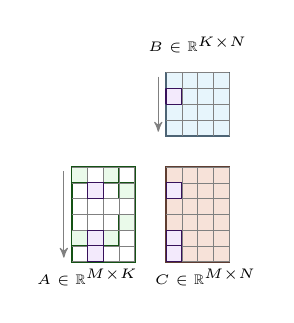
\begin{tikzpicture}
    % A
    \draw [thick,draw=LimeGreen!40!black] (.8,0) rectangle (1.6,1.2);
    \filldraw [fill=LimeGreen!10!white,draw=LimeGreen!40!black] (0.8+3*0.2,0+4*0.2) rectangle (0.8+3*0.2+0.2,0+4*0.2+0.2);
    \filldraw [fill=LimeGreen!10!white,draw=LimeGreen!40!black] (0.8+2*0.2,0+1*0.2) rectangle (0.8+2*0.2+0.2,0+1*0.2+0.2);
    \filldraw [fill=LimeGreen!10!white,draw=LimeGreen!40!black] (0.8+3*0.2,0+4*0.2) rectangle (0.8+3*0.2+0.2,0+4*0.2+0.2);
    \filldraw [fill=LimeGreen!10!white,draw=LimeGreen!40!black] (0.8+1*0.2,0+0*0.2) rectangle (0.8+1*0.2+0.2,0+0*0.2+0.2);
    \filldraw [fill=LimeGreen!10!white,draw=LimeGreen!40!black] (0.8+1*0.2,0+4*0.2) rectangle (0.8+1*0.2+0.2,0+4*0.2+0.2);
    \filldraw [fill=LimeGreen!10!white,draw=LimeGreen!40!black] (0.8+2*0.2,0+5*0.2) rectangle (0.8+2*0.2+0.2,0+5*0.2+0.2);
    \filldraw [fill=LimeGreen!10!white,draw=LimeGreen!40!black] (0.8+3*0.2,0+2*0.2) rectangle (0.8+3*0.2+0.2,0+2*0.2+0.2);
    \filldraw [fill=LimeGreen!10!white,draw=LimeGreen!40!black] (0.8+1*0.2,0+1*0.2) rectangle (0.8+1*0.2+0.2,0+1*0.2+0.2);
    \filldraw [fill=LimeGreen!10!white,draw=LimeGreen!40!black] (0.8+1*0.2,0+4*0.2) rectangle (0.8+1*0.2+0.2,0+4*0.2+0.2);
    \filldraw [fill=LimeGreen!10!white,draw=LimeGreen!40!black] (0.8+0*0.2,0+1*0.2) rectangle (0.8+0*0.2+0.2,0+1*0.2+0.2);
    \filldraw [fill=LimeGreen!10!white,draw=LimeGreen!40!black] (0.8+1*0.2,0+0*0.2) rectangle (0.8+1*0.2+0.2,0+0*0.2+0.2);
    \filldraw [fill=LimeGreen!10!white,draw=LimeGreen!40!black] (0.8+0*0.2,0+5*0.2) rectangle (0.8+0*0.2+0.2,0+5*0.2+0.2);
    \filldraw [fill=LimeGreen!10!white,draw=LimeGreen!40!black] (0.8+2*0.2,0+1*0.2) rectangle (0.8+2*0.2+0.2,0+1*0.2+0.2);
    \filldraw [fill=LimeGreen!10!white,draw=LimeGreen!40!black] (0.8+1*0.2,0+0*0.2) rectangle (0.8+1*0.2+0.2,0+0*0.2+0.2);
    %\filldraw [fill=LimeGreen!10!white,draw=LimeGreen!40!black] (.8,0) rectangle (1.6,1.2);
    \draw [step=0.4/2, very thin, color=gray] (.8,0) grid (1.6,1.2);
    
    \filldraw [fill=BlueViolet!10!white,draw=BlueViolet!40!black] (0.8+1*0.2,0+0*0.2) rectangle (0.8+1*0.2+0.2,0+0*0.2+0.2);
    \filldraw [fill=BlueViolet!10!white,draw=BlueViolet!40!black] (0.8+1*0.2,0+4*0.2) rectangle (0.8+1*0.2+0.2,0+4*0.2+0.2);
    \filldraw [fill=BlueViolet!10!white,draw=BlueViolet!40!black] (0.8+1*0.2,0+1*0.2) rectangle (0.8+1*0.2+0.2,0+1*0.2+0.2);

    \draw (1.0,-0.2) node {{\color{black}\tiny{$A\in\mathbb{R}^{\tiny{M \times K}}$}}};
  
    % Code Row-wise, iter 1
    %\draw [thick,draw=BlueViolet!40!black] (.8,1.0) rectangle (1.0,1.2);
    %\filldraw [fill=BlueViolet!10!white,draw=BlueViolet!40!black] (.8,1.0) rectangle (1.0,1.2);
    %\draw [step=0.4/2, very thin, color=gray] (.8,1.0) grid (1.0,1.2);
    %\draw[thin, draw=Gray, ->=, >=stealth'] (0.85, 1.3) -- (1.55, 1.3);

    % Code Col-wise, iter 1
    %\draw [thick,draw=BlueViolet!40!black] (.8,0) rectangle (1.0,1.2);
    %\filldraw [fill=BlueViolet!10!white,draw=BlueViolet!40!black] (.8,0) rectangle (1.0,1.2);
    %\draw [step=0.4/2, very thin, color=gray] (.8,0) grid(1.0,1.2);
    \draw[thin, draw=Gray, ->=, >=stealth'] (0.7, 1.15) -- (0.7, 0.05);

    %Code Inner Prod
    %\draw[thin, draw=Red] (.85, 1.1) -- (1.55, 1.1);
    %\draw[thin, draw=Gray, ->=, >=stealth'] (0.85, 1.3) -- (1.55, 1.3);

    % B
    \draw [thick,draw=Cerulean!40!black] (2,1.6) rectangle (2.8,2.4);
    \filldraw [fill=Cerulean!10!white,draw=Cerulean!40!black] (2,1.6) rectangle (2.8,2.4);
    \draw [step=0.4/2, very thin, color=gray] (2, 1.6) grid (2.8,2.4);
    
    \draw (2.4 , 2.75) node {{\color{black}\tiny{$B\in\mathbb{R}^{\tiny{K \times N}}$}}};
  
    % Code Row-wise, iter 1
    %\draw [thick,draw=BlueViolet!40!black] (2,2.2) rectangle (2.8,2.4);
    %\filldraw [fill=BlueViolet!10!white,draw=BlueViolet!40!black] (2,2.2) rectangle (2.8,2.4);
    %\draw [step=0.4/2, very thin, color=gray] (2, 2.2) grid (2.8,2.4);
    %\draw[thin, draw=Gray, ->=, >=stealth'] (2.05, 2.5) -- (2.75, 2.5);

    % Code Col-wise, iter 1
    \draw [thick,draw=BlueViolet!40!black] (2,2.2-0.2) rectangle (2.2-0.2,2.4-0.2);
    \filldraw [fill=BlueViolet!10!white,draw=BlueViolet!40!black] (2,2.2-0.2) rectangle (2.2,2.4-0.2);
    \draw[thin, draw=Gray, ->=, >=stealth'] (1.90, 2.35) -- (1.90, 1.65);
  
    %Code Inner Prod
    %\draw[thin, draw=Red] (2.1, 2.35) -- (2.1, 1.65);
    %\draw[thin, draw=Gray, ->=] (1.9, 2.35) -- (1.9, 1.65);

    % C
    \draw [thick,draw=BrickRed!40!black] (2,0) rectangle (2.8,1.2);
    \filldraw [fill=BrickRed!10!white,draw=BrickRed!40!black] (2,0) rectangle (2.8,1.2);
    \draw [step=0.4/2, very thin, color=gray] (2, 0) grid (2.8,1.2);


    % Code Row-wise, iter 1
    %\draw [thick,draw=BlueViolet!40!black] (2,1.0) rectangle (2.8,1.2);
    %\filldraw [fill=BlueViolet!50!white,draw=BlueViolet!60!black] (2,1.0) rectangle (2.8,1.2);
    %\draw [step=0.4/2, very thin, color=gray] (2, 1.0) grid (2.8,1.2);

    % Code Col-wise, iter 1
    %\draw [thick,draw=BlueViolet!40!black] (2,0) rectangle (2.2,1.2);
    %\filldraw [fill=BlueViolet!10!white,draw=BlueViolet!40!black] (2,0) rectangle (2.2,1.2);
    %\draw [step=0.4/2, very thin, color=gray] (2, 0) grid (2.2,1.2);

    %Code Inner Prod
    %\draw[thin, draw=Red] (2.05, 1.1) -- (2.15, 1.1);
    %\draw[thin, draw=Red] (2.1, 1.15) -- (2.1, 1.05);

    \filldraw [fill=BlueViolet!10!white,draw=BlueViolet!40!black] (2+0*0.2,0+0*0.2) rectangle (2+0*0.2+0.2,0+0*0.2+0.2);
    \filldraw [fill=BlueViolet!10!white,draw=BlueViolet!40!black] (2+0*0.2,0+4*0.2) rectangle (2+0*0.2+0.2,0+4*0.2+0.2);
    \filldraw [fill=BlueViolet!10!white,draw=BlueViolet!40!black] (2+0*0.2,0+1*0.2) rectangle (2+0*0.2+0.2,0+1*0.2+0.2);

    \draw (2.5 , -0.2) node {{\color{black}\tiny{$C\in\mathbb{R}^{\tiny{M \times N}}$}}};
\end{tikzpicture}
\end{document}
